\subsection{Security analysis and threat modeling TODO(is this professional wording for a report? not proofread yet)}
The section might suggest that the security analysis part of this project is over and done with. Have no allusions! This could not be far from the truth. The world of security in computing is a dubious cat-and-mouse game, and for non IT professionals a murky black art.  the group made this security analysis as a reminder that greater risk can come from an insecure implementation of this prototype. It is not uncommon for security to be lost and forgotten in the middle of development chaos and no one gives a second thought about security until there has actually been a security breach on an IT system.  The group felt that it is its professional duty , as a consultant, to  remind the customer  the risks associated and give a minute  indicator as to how this application could be abused and that security should be given as much gravity as functionality requirements. We could not emphasis more that this is by no means the end of the story.
\\[0.2cm]
In an environment where operation involves some inherent security risk, taking time to consider the security risks ahead of an actual crisis is well worth the effort. Having a web application can give one a greater audience, accessibility and scalable information dissemination platforms but at the same time it open wide a back door to your IT operations resources. Rogue code can create from minor inconvenience to completely crippling the system, causing a disruption in services. For web applications, it is incredibly hard to imagine where the security threat might come from or understand the motives of an attacker. Students trying to test their skill, IT vandalism or anyone looking for insight in to the internal operations of an organization can lurk in and wreak serious havoc unexpectedly.
\\[0.5cm]
There are two notable methods of security threat modeling techniques, Misuse case and Attack tree. Considering the nature of our project and the nature of content this application is going to deal with, and less sensitivity of the documents in the system, we opt to model our general security threats using Misuse case.
\begin{figure}[htb]
	\centering
    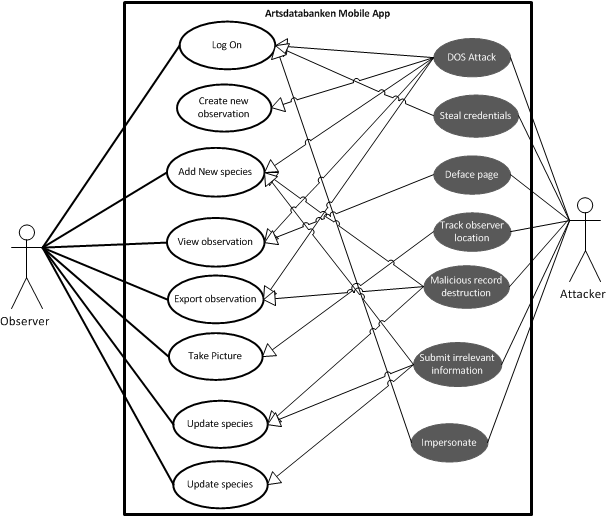
\includegraphics[width=0.9\textwidth]{reqspec/misusecase.png}
	\caption{Security threat model with Misuse case.}
	\label{fig:misusecase}
\end{figure}

\begin{table}[htb]
	\centering
    \begin{tabular}{| l | l |}
		\hline
		Potential threats & Mitigation suggestions \\
		\hline \hline
		Denial of service	& Thorough input validation \\& Clean exception handling \\
		Steal credentials	& Thorough input validation\\	& Strong authentication mechanism \\
        Deface content page & Thorough input validation\\
        Track observer location & Thorough input validation\\ & Clean picture meta-data\\ & Secure communication path\\
        Impersonate & Strong authentication\\
        Push irrelevant information & Thorough input validation\\
        Deliberate record destruction & Thorough input validation\\

		\hline
    \end{tabular}
  \caption{Threat mitigation suggestions}
\end{table}
